\section{Introduzione}
\subsection{Puntatori}
Gli indirizzi di memoria delle variabili sono interi (rappresentati in esadecimale) che conano i byte a partire dalla posizione 0x0000000. Gli indirizzi di memoria possono esere memorizazti in varibili come ogni altro intero.
\begin{definition}[Puntatori]
Andiamo così a definire le variabile che memorizzano indirizzi di memoria come \textbf{puntatori}, per distinguerli anche dagli altri tipi di variabili.
\end{definition}
\subsection{Operatori sui puntatori}
Sono due i principali operatori che possono essere usai con i puntatori.
\begin{itemize}
    \item \textbf{(\&)} \hspace{.1cm} - \hspace{.1cm} \textbf{Operatore indirizzo}. L'operatore di indirizzo è unario\footnote{Unario vuol dire che agisce un una sola varibile} e restituisce l'indirizzo di memoria dell'operando (può essere anche un altro puntatore, in questo caso restituisce l'indirizzo in cui è memorizzato il puntatore, cioè l'indirizzo di memoria di una variabile).
    \item \textbf{(*)} \hspace{.1cm} - \hspace{.1cm} \textbf{Operatore di indirezione o dereferenziazzione}. L'operatore di indirezione è unario e restituisce il valore dell'oggetto a cui punta l'operanda. 
\end{itemize}

\begin{note}
Nota che \& e * sono uno l'inverso dell'altro, quindi: \&*aPtr == *\&aPtr.
\end{note}

\begin{example}\label{esempio-1}
Di seguito un esempio di utilizzo di puntatori con anche i vari operatori.
\end{example}
\vspace{2pt}
\begin{lstlisting}[language=Javascript, caption=Esempio puntatori e operatori sui puntatori]
var a:Character = 'z', b:Character = 'h';
ref aPtr:Character = nil                        //0x0
aPtr = 0;                                       //0x0
aPtr = &a;                                      
print(&a, aPtr);                                //0x7ffeefbff60f, 0x7ffeefbff60f
print(*aPtr, a);                                //z, z
print(&aPtr);                                   //0x7ffeefbff60f
*aPtr = b;
print(*aPtr, a, b);                             //h, h, h
print(&b, &a, aPtr);                            // 3 volte 0x7ffeefbff60f
ref altro_aPtr:Character = &a;                  
print(altro_aPtr, *altro_aPtr);                 //0x7ffeefbff60f, h
\end{lstlisting}
\vspace{3pt}

\hspace{-15pt}\underline{Descrizione esempio:} Osservando l'esempio sopra \ref{esempio-1} possiamo vedere alle righe (11) e (12) che abbiamo una dichiarazione di un nuovo puntatore che punta alla stessa cella di memoria di "aPtr", abbiamo quindi più di un puntatore che punta alla stessa variabile.\\\\
Possiamo vedere che le locazioni di memoria sono numeri interi che individuano la posizione della cella di memoria (sono numeri interi scritti in esadecimale, ma sempre numeri interi), è quindi possibili effettuare operazioni aritmetiche sui puntatori, cioè è possibile manipolare tramite operazioni aritmetiche le locazioni.\\
\begin{example}
Se per esempio prendiamo un ambiente ed una memoria così composti:
\end{example}
\begin{wrapfigure}[10]{r}{8cm}
    \vspace{-5pt}
    \centering
    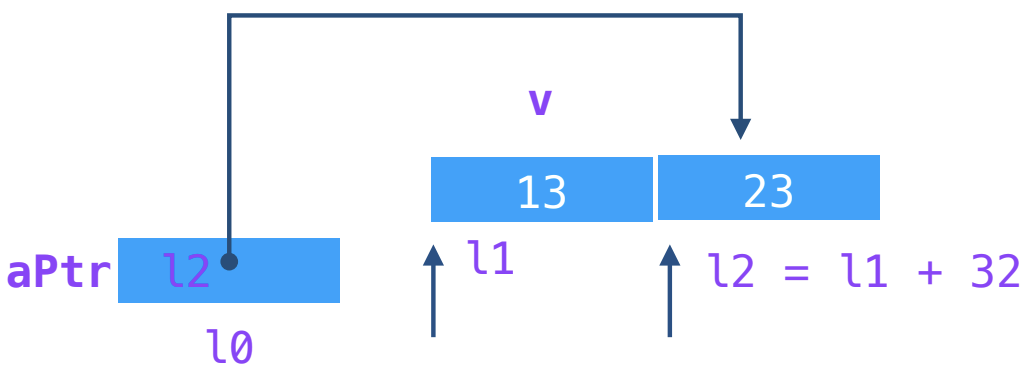
\includegraphics[width=7cm]{images/esempio-puntatori-1.png}
    \caption{Operazioni algebriche su puntatori}
\end{wrapfigure}

$\rho = [(aPtr, l2)]$ \: \: $\sigma = [(l1,13), (l2,23)]$\\ \\
Abbiamo quini un puntatore "aPtr" che punta alla locazione l1, il quale contiene il numero 13, più una posizione l2, successiva alla l1, che contiene 23.\\ Se ipotizziamo che il nostro sistemi archivi le informazioni con una base di 32 bit \footnote{Questo vuol dire che ogni vaore è salvato con 32 bit, quindi ogni 32 ci sarà un nuovo valore archiviato} ed andiamo a sommare 32 a "aPtr" succederà che ci sposteremo di 32 posti nella memoria raggiungendo l2, quindi "aPtr" = l2.

\subsection{Strutture dati}
\begin{definition}[Struttura dati]
Una \textbf{struttura dati} è un formato che serve ad organizzare e memorizzare dati in modo da renderli agevolmente disponibili agli algoritmi che li manipolano.
\end{definition}
\hspace{-15pt}Alcune caratteristiche delle strutture dati:
\begin{itemize}
    \item Una struttura dati è detta \textbf{omogenea} se contiene dati tutti dello stesso tipo. Altrimenti è \textbf{disomogenea}.
    \item Una struttura dati è \textbf{statica} se la sua dimensione non varia durante l'esecuzione del programma. Altrimenti è detta \textbf{dinamica}.
    \item Una struttura dati è \textbf{lineare} se i dati sono organizzati come sequenze di valori. Altrimenti è detta \textbf{non lineare}.
\end{itemize}
Una struttura dati è inoltre caratterizzata dalle operazioni elementari disponibili per inserire, reperire e modificare i dati che memorizza.

\subsection{Notazione asintotica}
Quando andiamo a scrivere un algoritmo, per calcolare il costo di tale algoritmo, bisogna andare a fare una serie di assunzioni che appunto facciamo basandoci sul fatto che stiamo lavorando su una macchina astratta, quindi con caratteristiche fissate.
\begin{itemize}
    \item L'accesso alle celle di memoria avviene in tempo costante.
    \item Le operazioni aritmetiche e logiche della ALU avvengono in tempo costante.
    \item Gli assegnamenti avvengono in tempo constante.
    \item I controlli del flusso (salti, assegnamento al registro PC) avvengono in tempo costante.
\end{itemize}
Noi per andare a calcolare il costo degli algoritmi si possono utilizzare due modelli di calcolo:
\begin{enumerate}
    \item \textbf{Word model:} tutti i dati occupano solo una cella di memoria.
    \item \textbf{Bit model:} unità elementare di memoria bit, si usa quanto le grandezze sono troppo grandi.
\end{enumerate}

\hspace{-15pt}Esistono una serie di parametri da analizzare quando scriviamo una algoritmo, essi infatti permettono di garantire il suo corretto funzionamento, e o la sua ottimizzazione, essi sono i seguenti.
\begin{itemize}
    \item \textbf{Complessità:} Può essere sintetizzato con l'analisi dell'utilizzo delle risorse che sarebbero: tempo di esecuzione, spazio di memoria, banda di comunicazione.
    \item \textbf{Correttezza:} Indica se l'algoritmo fa quello per cui è stato progettato, e si fa tramite una \underline{dimostrazione formale} il quale permette di dimostrare la correttezza andando a risolvere tutte le istanze del problema, o una \underline{ispezione formale}, quest'ultima spesso ha che fare con la struttura de programma e si usano metodi come il testing o il profalig, il primo prevede di provare il programma nelle situazioni critiche, il secondo analizza il tempo che la CPU elabora una determinata parte del programma.
    \item \textbf{Semplicità:} Questo paramento indica se l'algoritmo è facile da capire e manutenere e si fa tramite identificatori significativi, algoritmo ben commentato, strutture dati adeguate, rispetto degli standard.
\end{itemize}

\begin{definition}[Complessità di un problema]
    La complessità di un problema P è la complessità del miglior algoritmo A che lo risolve.
\end{definition}
Per andare a trovare la complessità del problema partiamo dal fatto che, preso un algortimo A, la complessità di A determina un limite superiore alla complessità di P (cioè quando si verifica il caso peggiore uso A per risolvere P).\\
Se riusciamo a determinare un limite inferiore $g(n)$ per P, per ogmo algoritmo A che risolve P ho che $A \in \Omega(g(n))$, dove $g(n)$ è il minimo numero di operazione che posso impiegare per risolvere P. Quindi possiamo dire che:
\begin{center}
    $A \in \Theta(g(n)) \Longrightarrow$ A ottimo \footnote{Ricorda che dire che $A \in \Theta(g(n))$ vuol dire che $A \in O(g(n))$ e $A \in \Omega(g(n))$}
\end{center}
Per fare ciò quindi bisogna anche ad andare a calcolare il limite inferiore del caso pessimo, e ciò e possibile tramite 3 metodi: la \textbf{dimensione dei dati}, gli \textbf{eventi contabili} e gli \textbf{alberi decisionali}.

\begin{itemize}
    \item \textbf{Dimensioni dei dati:} Se la soluzione di un problema richiede l'esame di tutti i dati in input, allora $\Omega(n)$ è un limite inferiore.
\end{itemize}
\begin{example}
    Sommare tutti gli elementi di un array.
\end{example}
\begin{itemize}
    \item \textbf{Eventi contabili:} Se la soluzione di un problema richiede la ripetizione di un certo evento, allora il numero di volte che l'evento si ripete (moltiplicato per il suo costo) è un limite.
\end{itemize}
\begin{example}
    Se voglio costruire un array i cui elementi sono la radice quadrata degli elementi di un array dato, dovrò fare un ciclo che scorre l'array dato e applica la radice quadrata. Gli eventi contabili sono quindi il numero di iterazioni.
\end{example}

\subsection{Big-O notation}
La notazione Big O ha molteplici scopi della scritture di un algoritmo.
\begin{itemize}
    \item Serve a rappresentare la complessità relativa di un algoritmo.
    \item Descrive le prestazioni di un algoritmo e come queste scalano al cresce dei dati in input.
    \item Descrive un limte superiore al tasso di crescita di na funzione ed il caso peggiore.
\end{itemize}

\subsubsection{Limite superiore asintotico}
\begin{definition}[Limite superiore asintotico]
Il limite superiore asintotico si definisce come:
\begin{center}
    $O(g(n)) = \{f(n) \: |\: \exists c, n_0 > 0 \: . \: \forall n > n_0, 0 \leq f(n) \leq c \cdot g(n)\}$
\end{center}
\end{definition}
\hspace{-15pt}Si scrive come $f(n) \in O(g(n))$ oppure $f(n) = O(g(n))$ e si legge $f(n)$ è nell'ordine $O$ grande di $g(n)$.
\begin{example}
Esempio di calcolo del limite superiore asintotico
\end{example}
\begin{wrapfigure}[7]{l}{8cm}
    \vspace{-15pt}
    \centering
    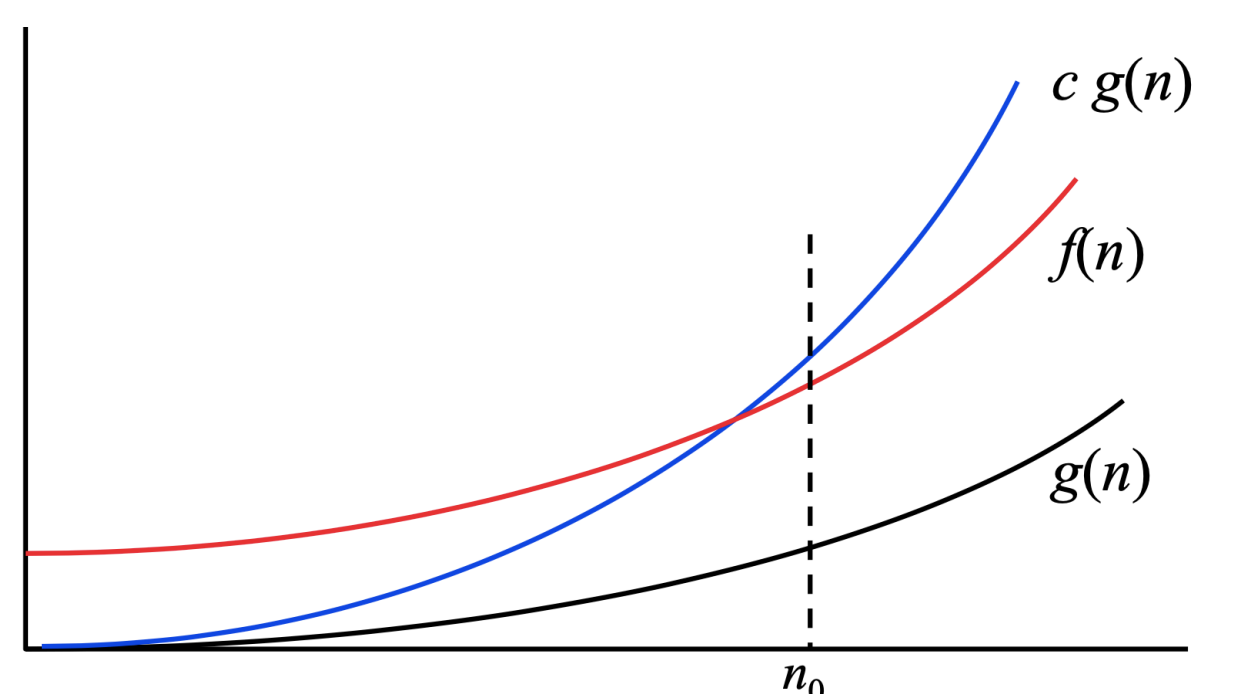
\includegraphics[width=6cm]{images/limite-superiore-asintotico.png}
    \vspace{-5pt}
    \caption{Limite superiore asintotico}
\end{wrapfigure}
Prendiamo due funzioni e determiniamo i punti $n_0$ e $c$ per cui è soddisfatta la definizione.
\begin{center}
    \vspace{-5pt}
    $f(n) = 3n^2 + 5$ \: \: \: $g(x)=n^2$
\end{center}
Stabiliamo un $c = 4$ e $n_0 = 3$.
\begin{enumerate}
    \item $4 \cdot g(n) = 4n^2 = 3n^2 + n^2 $
    \item $3n^2 + n^2 \geq 3n^2 + 9 $ (per ogni $n \geq 3$)
    \item $3n^2 + 9 > 3n^2+5 \Longrightarrow 4 \cdot g(n) > f(n)$
\end{enumerate}

\subsubsection{Limite inferiore asintotico}
\begin{definition}[Limite inferiore asintotico]
Il limite inferiore asintotico si definisce come:
\begin{center}
    $\Omega(g(n)) = \{f(n) \: |\: \exists c, n_0 > 0 \: . \: \forall n > n_0, 0 \leq c \cdot g(n) \leq f(n) \}$
\end{center}
\end{definition}
\hspace{-15pt}Si scrive come $f(n) \in \Omega(g(n))$ oppure $f(n) = \Omega(g(n))$ e si legge $f(n)$ è nell'ordine $\Omega$ grande di $g(n)$.
\begin{example}
Esempio di calcolo del limite inferiore asintotico. Prendiamo due funzioni e determiniamo i punti $n_0$ e $c$ per cui è soddisfatta la definizione.
\end{example}
\begin{wrapfigure}[6]{r}{8cm}
    \vspace{-15pt}
    \centering
    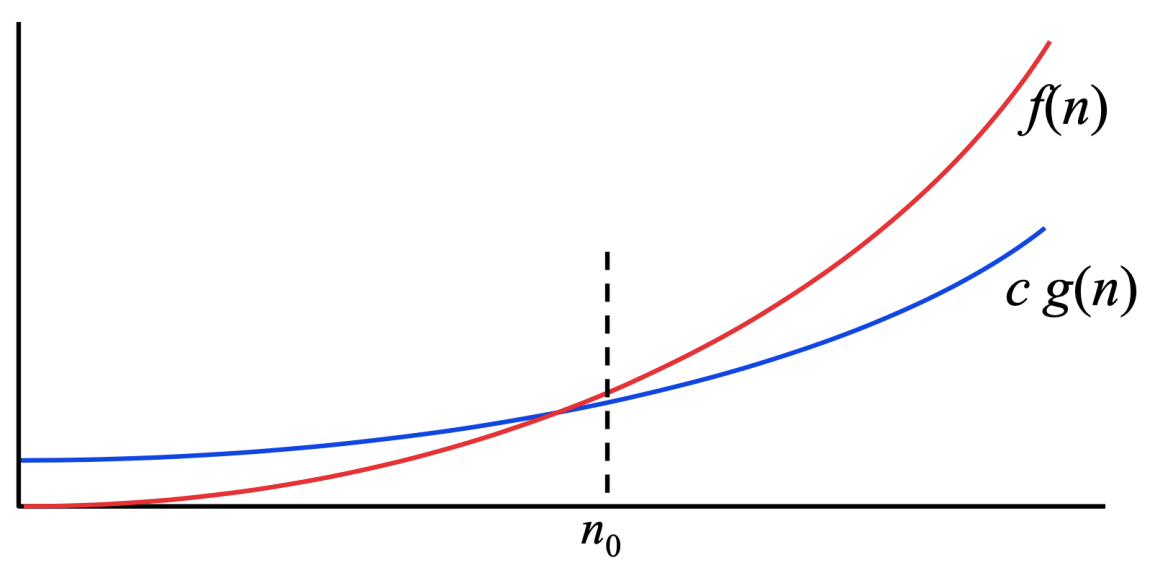
\includegraphics[width=6cm]{images/limite-inferiore-asintotico.png}
    \vspace{-5pt}
    \caption{Limite superiore asintotico}
\end{wrapfigure}

$f(n) = \frac{n^2}{2}-7$ \: \: \: $g(x)=n^2$\\
Stabiliamo un $c = 4$ e $n_0 = 3$.
\begin{enumerate}
    \item $\frac{1}{4} \cdot g(n) = \frac{n^2}{4} = \frac{n^2}{2} - \frac{n^2}{4}$
    \item $\frac{n^2}{2} - \frac{n^2}{4} \leq \frac{n^2}{2} - 9 $ (per ogni $n \geq 6$)
    \item $\frac{n^2}{2} - 9 > \frac{n^2}{2}-7 \Longrightarrow \frac{1}{4} \cdot g(n) < f(n)$
\end{enumerate}

\subsubsection{Limite asintotico stretto}
\begin{definition}[Limite inferiore asintotico]
Il limite asintotico stretto si definisce come:
\begin{center}
    $\Theta(g(n)) = \{f(n) \: |\: \exists c_1, c_2, n_0 > 0 \: . \: \forall n > n_0, 0 \leq c_1 \cdot g(n) \leq f(n) \leq c_2 \cdot g(n) \}$
\end{center}
\end{definition}
\begin{wrapfigure}[5]{r}{8cm}
    \vspace{-10pt}
    \centering
    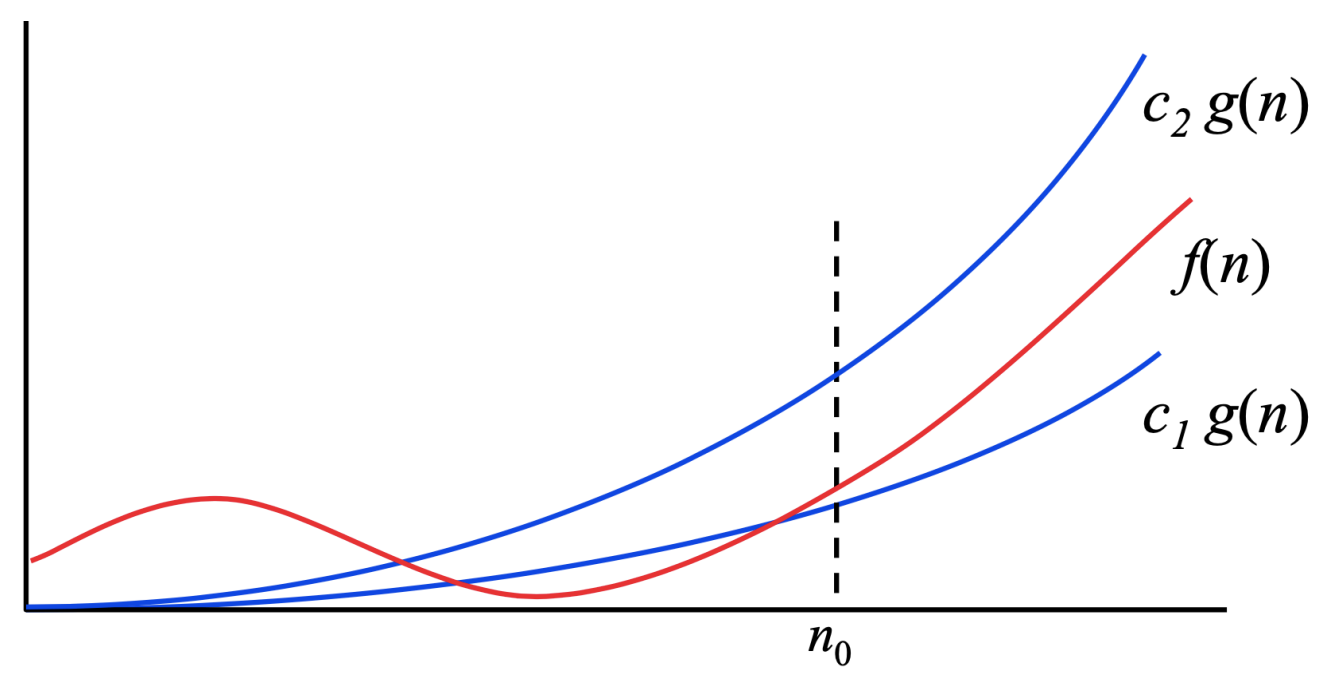
\includegraphics[width=6cm]{images/limite-asintotico-stretto.png}
    \vspace{-5pt}
    \caption{Limite asintotico stretto}
\end{wrapfigure}
Si scrive come $f(n) \in \Theta(g(n))$ oppure $f(n) = \Theta(g(n))$ e si legge $f(n)$ è nell'ordine $\Theta$ grande di $g(n)$.\\\\
Dalla definizione deriva che:\\
$f(n) \in \Theta(g(n)) \Longleftrightarrow f(n) \in \Omega(g(n)) \land f(n) \in O(g(n))$\\


\subsubsection{Teoremi sulla notazione asintotica}
\begin{theorem}
Per ogni $f(n)$ e $g(n)$ vale che:
\begin{enumerate}
    \item $f(n) = O(g(n)) \Longleftrightarrow g(n) = \Omega(f(n))$
    \item Se $f_1(n) = O(f_2(n)) \land f_2(n) = O(f_3(n)) \Longrightarrow f_1(n) = O(f_3(n))$
    \item Se $f_1(n) = \Omega(f_2(n)) \land f_2(n) = \Omega(f_3(n)) \Longrightarrow f_1(n) = \Omega(f_3(n))$
    \item Se $f_1(n) = \Theta(f_2(n)) \land f_2(n) = \Theta(f_3(n)) \Longrightarrow f_1(n) = \Theta(f_3(n))$
    \item Se $f_1(n) = O(g_1(n)) \land f_2(n) = O(g_2(n)) \Longrightarrow O(f_1(n) + f_2(n)) = O(max\{g_1(n),g_2(n)\})$
    \item Se $f(n)$ è un polinomio di grafo $d \Longrightarrow f(n) = \Theta(n^d)$
\end{enumerate}
\end{theorem}

\subsubsection{Limite superiore asintotico non stretto}
\begin{definition}[Limite superiore asintotico non stretto]
Il limite superiore asintotico non strettosi definisce come:
\begin{center}
    $o(g(n)) = \{f(n) \: |\: \forall c \: \exists n_0 > 0 \: . \: \forall n > n_0, 0 \leq f(n) \leq c \cdot g(n) \}$
\end{center}
\end{definition}
\hspace{-15pt}Si scrive come $f(n) \in o(g(n))$ oppure $f(n) = o(g(n))$ e si legge $f(n)$ è nell'ordine $o$ piccolo di $g(n)$.\\
$f(n)$ è limitata superiormente da $g(n)$, ma non la raggiunge mai.\\
\begin{wrapfigure}[7]{l}{7cm}
    \vspace{-15pt}
    \centering
    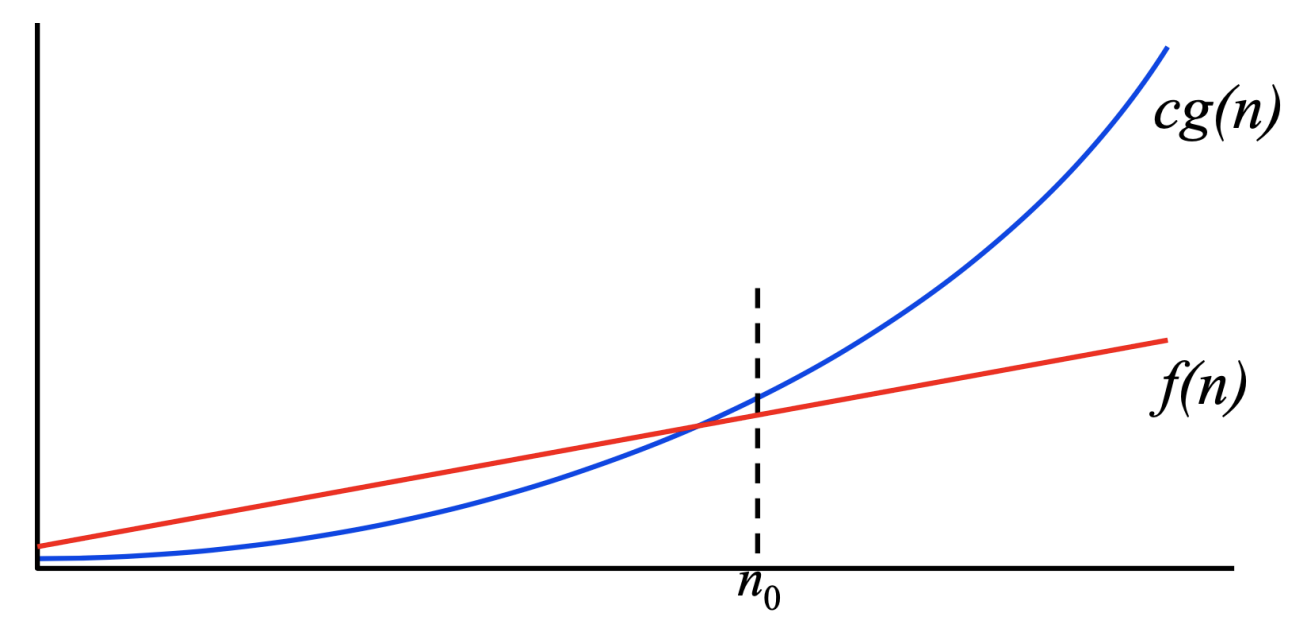
\includegraphics[width=6.5cm]{images/limite-superiore-asintotico-non-stretto.png}
    \vspace{-5pt}
    \caption{Limite superiore non stretto}
\end{wrapfigure}

\vspace{-15pt}
E immediato dalla definizione che:
\begin{center}
    $o(g(n)) \Longrightarrow O(g(n))$
\end{center}
Non vale il viceversa: 
\begin{center}
    $2n^2 \in O(n^2) \land 2n^2 \notin o(n^2)$
\end{center}
Definizione alternativa:
\begin{center}
    $f(n) \in o(g(n)) \Longleftrightarrow \lim\limits_{n\to \infty}\frac{g(n)}{f(n)} = \infty$
\end{center}

\subsubsection{Limite inferiore asintotico non stretto}
\begin{definition}[Limite inferiore asintotico non stretto]
Il limite inferiore asintotico non stretto si definisce come:
\begin{center}
    $\omega(g(n)) = \{f(n) \: |\: \forall c \: \exists n_0 > 0 \: . \: \forall n > n_0, 0 \leq c \cdot g(n) \leq f(n) \}$
\end{center}
\end{definition}
\hspace{-15pt}Si scrive come $f(n) \in \omega(g(n))$ oppure $f(n) = \omega(g(n))$ e si legge $f(n)$ è nell'ordine $\omega$ piccolo di $g(n)$.\\
$f(n)$ è limitata inferiormente da $g(n)$, ma non la raggiunge mai.\\
\begin{wrapfigure}[7]{l}{7cm}
    \vspace{-15pt}
    \centering
    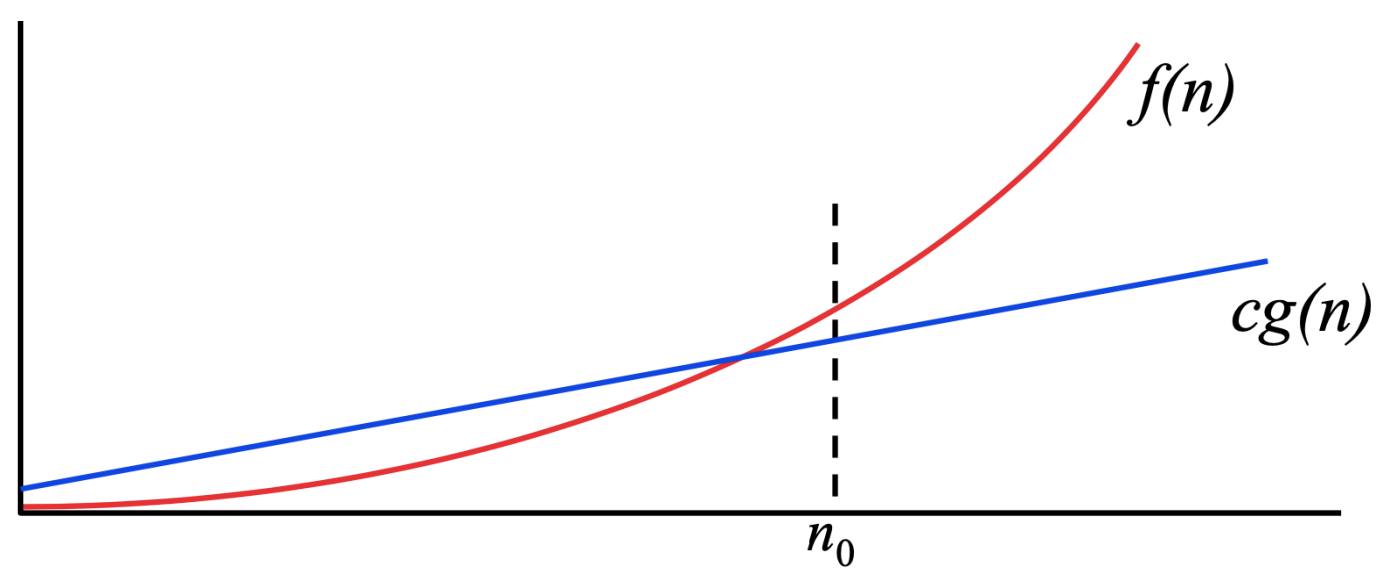
\includegraphics[width=6.5cm]{images/limite-inferiore-asintotico-non-stretto.png}
    \vspace{-5pt}
    \caption{Limite asintotico stretto}
\end{wrapfigure}

\vspace{-15pt}
E immediato dalla definizione che:
\begin{center}
    $\omega(g(n)) \Longrightarrow \Omega(g(n))$
\end{center}
Non vale il viceversa: 
\begin{center}
    $\frac{1}{5}n^2 \in \Omega(n^2) \land \frac{1}{2}n^2 \notin \omega(n^2)$
\end{center}
Definizione alternativa:
\begin{center}
    $f(n) \in \omega(g(n)) \Longleftrightarrow \lim\limits_{n\to \infty}\frac{g(n)}{f(n)} = 0$
\end{center}
